\chapter{Umsetzung}
\section{Fahren}
Da der \textit{EarthROVER} mit vier Ketten fahren soll bedarf es hier einer besonderen Lösung. Um vier Motoren an einem \textit{NXT-Brick} zu verwenden zu können werden zwei Motoren(auf einer Seite) mit Hilfe von RCX-Motorkabeln verbunden. Hierzu werden drei RCX-Kabel verwendet. Das erste Kabel wird in den NXT gesteckt. An das andere Ende wird ein zweites RCX-Kabel aufgesteckt. Ein drittes Kabel wird verkehrt herum aufgesteckt. Hierdurch werden beide Motoren entgegengesetzt drehen. Da bei unserem Aufbau auf der Basis die Motoren auf einer Seite entgegensetzt sind passt das so genau. 

\begin{capfigure}[RCX-Kabel]
	 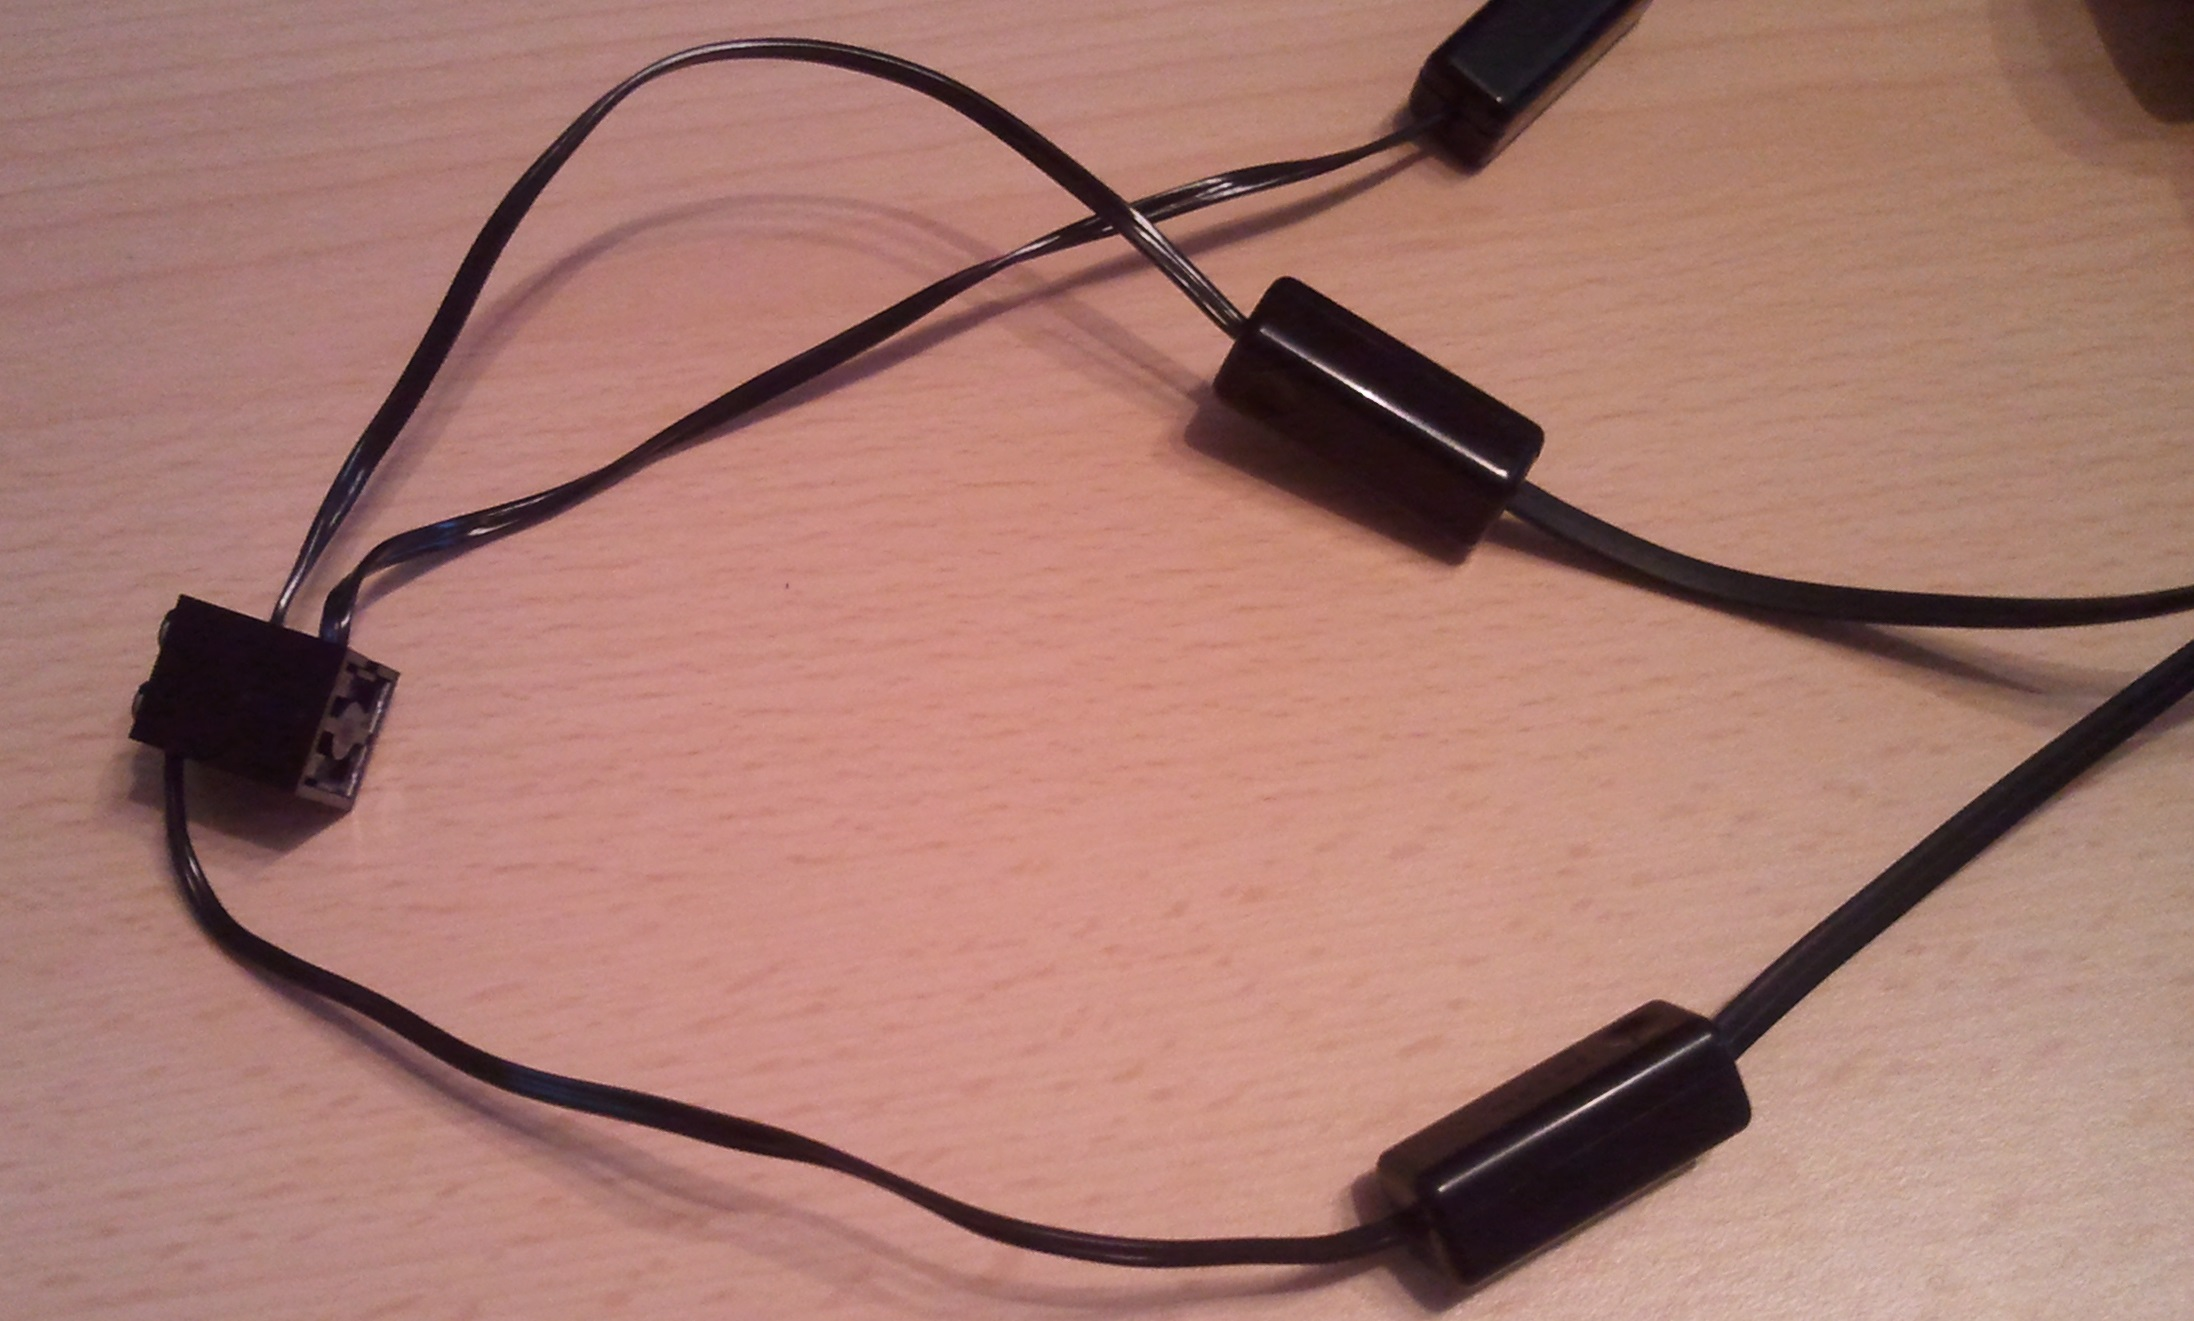
\includegraphics[width=\textwidth]{images/implementation/rcxcables}
\end{capfigure}

Zu Beachten ist hierbei, dass durch die Benutzung der RXC-Kabel die Motoren keine Tachowerte mehr liefern. Man kann die Motoren als nicht reguliert verwenden und auch keine Tachowerte auslesen.

Dies stellt in unserem Szenario allerdings kein Problem dar, da es für das Fahren bei unserer Konstruktion ausreicht bei einem der vier Motoren in der Lage zu sein den Motor reguliert zu betreiben.

Da wir was die Anzahl der Sensoren betrifft eingeschränkt sind und somit lediglich einen Ultraschallsensor zum Fahren verwenden haben wir uns dazu entschieden diesen an der linken Seite anzubringen. Beim der Erkundung fährt der \textit{EarthROVER} entweder geradeaus oder er dreht sich nach rechts. Da der Ultraschallsensor an der linken Seite angebracht ist können wir so besser vermeiden, dass der Roboter hängen bleibt.

\subsection{Orientierung}
Zur Orientierung verwendet der \textit{EarthROVER} Kompass-werte. Um Fehlmessungen des Kompass abzuschwächen wurde ein Kalmanfilter verwendet. Für den Kalmanfilter wird neben dem \textit{HiTechnic Compass Sensor} noch ein \textit{HiTechnic Gyro Sensor} verwendet.

Der Kalmanfilter korrigiert den Wert des Kompasses anhand der gemessenen Beschleunigung des Gyro-Sensors. Die Veränderung der Werte wird geglättet und ist somit präziser.

Neben dem eigentlichen Kalmanfilter werden die gelesenen Werte der beiden Sensoren vor dem Filtern über einen kurzen Zeitraum gemittelt um Ausreißer auszugleichen.

Es sei noch zu erwähnen, dass die Sensoren sehr anfällig auf Interferenzen von Magnetfeldern sind. Selbst der \textit{NXT-Brick} beeinflusst bereits den Sensor. Daher sind die Werte auch gefiltert nicht genau und weichen je nach Umgebung stark von der Realität ab.

\subsection{Weg merken}
Damit der \textit{EarthROVER} sich den Weg möglichst präzise Merken kann haben wir uns dazu entschieden, dass der \textit{EarthROVER} sich entweder geradlinig bewegt oder auf der Stelle dreht. Er kann also keine Kurven fahren. Dies hat den Vorteil, dass wir präzise Werte haben um den Weg aufzuzeichnen.

Der \textit{EarthROVER} merkt sich zwei Arten von Bewegungen:
\begin{capitemize}[Bewegungsarten]
	\item Geradlinig Fahren: Umdrehungen und Fahrtrichtung wird aufgezeichnet
	\item Auf der Stelle drehen: Mit Hilfe des gefilterten Kompasses wird die Differenz zwischen Startwinkel und Endwinkel und die Drehrichtung aufgezeichnet.
\end{capitemize}

\subsection{Zurück fahren}
Um den \textit{EarthROVER} wieder zu seinem Startpunkt zu bringen haben wir zwei Optionen vorgesehen. Umsetzen konnten wir nur die \nameref{lbl:simplemethod}.

\subsubsection{Simple Methode}
\label{lbl:simplemethod}
Bei der simplen Methode fährt der \textit{EarthROVER} den Weg genau so wieder zurück wie er ihn gefahren ist. Dazu geht er einfach die aufgezeichneten Schritte in umgekehrter Reihenfolge durch und führt die umgekehrte Aktion durch(Anstelle von Vorwärts Rückwärts, etc.).

\subsubsection{Direkte Methode}
Bei der direkten Methode sollte der \textit{EarthROVER} den direkten Weg zum Ausgangspunkt fahren. Um dies zu erreichen wird nach jeder zurückgelegten Fahrtbewegung(Vorwärts bzw. Rückwärts) der direkte Weg berechnet. Hierzu wird sich der allgemeine Kosinussatz zur Hilfe genommen.

\begin{capdefinition}{Allgemeiner Kosinussatz}
	Formeln:
	
	$c^2 = a^2 + b^2 - 2ab*cos(\gamma)$
	
	$b^2 = a^2 + c^2 - 2ac*cos(\beta)$
\end{capdefinition}

\begin{capfigure}[Kosinussatz]
	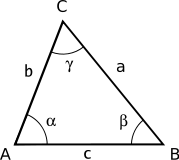
\includegraphics[width=5cm]{images/implementation/cosinus}
\end{capfigure}

Die Berechnung beginnt ab der zweiten Fahrbewegung. $A$ stellt den Startpunkt dar. Die erste Fahrbewegung ist $b$, die erste Drehbewegung ist $\gamma$ und die zweite Fahrbewegung ist $a$. Um aus dieser Position zurück zu gelangen muss zum einen $c$ und zum Anderen $\beta$ bekannt sein.

Um $c$ zu berechnen müssen wir lediglich die obere Formel wie folgt umstellen:

$c = \sqrt[2]{a^2 + b^2 - 2ab*cos(\gamma)}$

Damit haben wir unser $c$, jetzt fehlt noch unser $\beta$. Hierfür wird die zweite Formel verwendet. Wir stellen diese wie folgt um:

$\beta = arcos((a^2 + c^2 - b^2)2ac)$

Nun können wir auch unser $\beta$ berechnen. Damit haben wir alles um zum Ausgangspunkt zurück zu fahren.

Für den nächsten Schritt werden dann wie folgt die Werte zugewiesen:\\
\\
\begin{tabular}[htbp]{|l|l|}
	\hline
	Neue Werte & alte Werte \\
	\hline
	$b$ & $c$ \\
	\hline
	$a$ & Fahrstrecke des nächsten Schritts \\
	\hline
	$\gamma$ & $180° - \beta$\\
	\hline
\end{tabular}

Auf diese Art kennt der \textit{EarthROVER} zu jeder Zeit den direkten Weg zum Ausgangspunkt. Diese Variante hat einen deutlich kürzeren Weg als die erste Variante.

Hätten wir die Erkennung und Aufzeichnung von Hindernissen implementiert müsste natürlich an dieser Stelle noch sichergestellt werden, dass auf dem Weg kein Hindernis ist. Zudem könnten auf dem direkten Weg bisher unbekannte Hindernisse auftreten.

\section{Ball finden}
Damit sich der Ball von regulären Objekten unterscheiden lässt wird ein Infrarotball verwendet. Um diesen zu finden benutzen wir den \textit{HiTechnic Infrared Seeker}.

\begin{capfigure}[HiTechnic Infrared Seeker - Sensoren]
	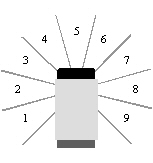
\includegraphics[width=5cm]{images/implementation/irseeker}
\end{capfigure}

Wie auf der Abbildung zu sehen ist liefert der Sensor neun Werte. Um den Ball zu finden muss man dafür sorgen, dass der Wert 5 am stärksten ist. Dazu fährt der \textit{EarthROVER} zuerst normal und sucht die Umgebung ab, sobald er eines der neun Signale den Ball bemerkt stoppt er den normalen Suchmodus und steuert von nun an über den \textit{HiTechnic Ifrared Seeker}.

Von hier an dreht sich der Roboter immer solange bis der Wert 5 das stärkste Signal liefert. Dann fährt er auf das Signal zu und korrigiert bei Bedarf die Richtung. Sobald er in der passenden Entfernung zum Ball ist kann der Greifarm den Ball dann aufheben.

\section{Greifarm}
\TODO{Für Jan: ergänzen}

\section{Raspberry Pi}

Im Ursprünglichen Konzept sollte der Raspberry Pi eine zentrale Rolle für den Rover spielen. Jedoch wurden durch technische Probleme nur eine einfachere Lösung realisiert.

\subsection{Ursprüngliche Konzeption} 

Das Urprüngliche Konzept sah vor, dass der über ein Raspberry PI ein WLAN aufgespannt wird über deren Kameramodul ein Livebild übertragen wird, man die aktuellen Werte der Sensoren auslesen kann und einige Remotefunktionen als Fernsteuerung ausführen.

\subsection{Technische Schwierigkeiten}

Bei der Umsetzung gab es einige technische Schwierigkeiten, die leider nicht gelöst werden konnten.

\subsubsection{Ansteuerung über den Raspberry Pi}

Wie im ursprünglichen Konzept vorgesehen, wollten wir die NXT per über USB an den Raspberry Pi anschließen und ansteuern. Als Programmiersprache wurde dazu NXT-Python ausgewählt. Dadurch was es auch nicht möglich, die Daten der Sensoren auf den Webserver zu übertragen.

\subsubsection{Kameramodul}

Zur Übertragtung des Videostreams wurde, das für den Raspberry Pi selbst entwickelte Kameramodul ausgewählt. Dabei stellte sich schnell heraus, dass die Möglichkeiten und Ansteuerungen dieses Moduls bei weitem nicht die Leistungsfähigkeit haben, wie Ansteuerungsmöglichkeiten einer normalen USB Kamera. Aus diesem Grund wurde eine normale USB Kamera ausgewählt.

\subsection{Umsetzung}

Aufgrund der Einschränkungen wurde nur eine einfachere Lösung implementiert. Zuerst wurde die Möglichkeit geschaffen sich per Browser ein Livebild


Der Raspberry PI baut dabei ein WLAN auf, streamt ein Livebild einer USB Kamera mit Hilfe des Webservers und liefert die Möglichkeit die Fahrt des Rovers per Browser zu verfolgen.

\subsection{Verbesserungs Möglichkeiten}
